\documentclass[a4paper,12pt]{article}

\usepackage[pdftex]{graphicx}

\title{Summa Metadata Storage}
\author{bam}

\begin{document}

\maketitle

%INTRODUCTION (SUMMARY)

The Summa Metadata Storage is accessed through the \texttt{Access}
interface.  There are two implementations of this interface. One is
based on a postgresql database and the other is based on a Lucene
index and is almost identical to the 'Netmusik' Metadata Storage. The
\texttt{Access} interface has been changed quite a bit, as the delete
method now changes the state of the record to deleted, but keeps the
record in storage; a new method has been introduced to remove the
records which were marked deleted before a given time; and the records
now have a base attribute (the origin of the record).

\section{Component Interface}

The \texttt{Access} interface provides methods for creating,
updating and deleting records in the database and for retrieving
records and iterators over a collection of records.
 
%\vspace{5mm}
%\noindent
%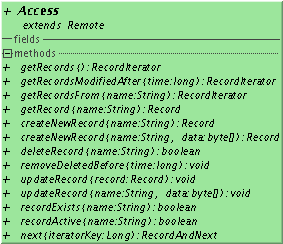
\includegraphics[width=.6\textwidth]{Access.png}

%\vspace{5mm}
%\noindent
A few important interpretation decisions:
\begin{itemize}
\item{\texttt{deleteRecord} changes the state of the record to
  \texttt{DELETED}.}
\item{\texttt{recordExists} is true if the record exists in storage
  (may have state \texttt{DELETED}).}
\item{\texttt{recordActive} is true if the record exists in storage
  \emph{and} does not have state = \texttt{DELETED}.}
\item{\texttt{createNewRecord} with a given id is possible if and only
if \texttt{!recordActive} for this id, i.e. we can create a new record
if no record with this id exists or if the existing record has state =
\texttt{DELETED}.}
\item{\texttt{removeDeletedBefore} a given time will remove all
  records marked \texttt{DELETED} before the given time.}
\end{itemize}

See the javadoc for further introduction to the different methods. The
classes \texttt{Record} and \texttt{RecordIterator} are used for
returning results. \texttt{Record} has been extended with a state and
a base, which means that the record now holds an id, a content, a
'last update time stamp', a state and an original base. Only the
content can be changed in a record object. The state is either
standard or deleted. The \texttt{RecordIterator} is a remote
iterator. It can be used like any other iterator, but it will make a
remote call for each use of the \texttt{next()} method.
 
\section{Lucene Index Storage}

A few introductory notes:

\begin{itemize}
\item{When moving or restarting the storage server, remember to update
\texttt{controllucene.properties} (\texttt{directory\_name} and
\texttt{create\_new\_index}).}
\item{On restart also remember to check (in \texttt{/tmp/}) if there
  is an old write lock and delete it.}
\item{If you want to use IDEA for testing, remember to add the
  \texttt{config} directory to the module libraries in project settings.}
\end{itemize}

The class \texttt{ControlLucene} implements the \texttt{Access}
interface as well as the \texttt{ControlLuceneMBean}, which makes
adjusting of the Lucene storage possible.

\subsection{Internal Design}

The implementation has been updated to match the Lucene 1.9.1 API,
some correction have been made and some Lucene index parameters have
been made available through the MBean.

\texttt{ControlLucene} has been designed to postpone the flushing of
add operations and the performance of delete operations and do these
in batches.

It may still be possible to optimise further. Updating the same record
repeatedly is currently very expensive, but I'm guessing we will
rarely do this. Updating a number of different records allows us to
collect the remove and add operations into batches. Retrieving an
iterator is also expensive as it requires first closing the writer
(saving all add operations), then saving all remove operations and
then closing the writer again to save the add operations created by
the \texttt{saveRemoves} method.

\subsection{Testing}

The class \texttt{LuceneStorageServer} starts the Lucene Storage as an
\texttt{Access} server, and the class \texttt{LuceneTestClient} should
test all methods available from the \texttt{Access} interface. The
methods available from the MBean interface can be tested from
\texttt{jconsole} (not if the storage is started from IDEA).

Wed May 03: The small test class has revealed problems, and these have
been fixed. The large scale test will probably be done by the Ingest
module; unfortunately not before.

\subsection{System Requirements and Installation}

The Ant build file should provide us with a \texttt{lucenestorage.tgz}
file in the \texttt{dist} directory. This includes the
\texttt{luceneStorage.sh} script for starting the storage server. The
RMIServer and ports should be set in \texttt{luceneStorage.sh}. The
storage properties should be set in
\texttt{config/controllucene.properties}, and the log properties
should be set in \texttt{config/log4j.xml}.

\section{Postgres Database Storage}

TODO

\section{Alternatives, Discussion and Further Work}

Regardless of the chosen storage, we might want to change return type
of the update methods in the \texttt{Access} interface to boolean.

We might want to change \texttt{Access} to extend the \texttt{Map}
interface, in which case we get a \texttt{put} method, which will
always put the given \texttt{Record} (content) into storage associated
with the given id (key) and return the 'old' record associated with
this id (null if there was no record with this id).

\end{document}
